\documentclass[11pt, % The default document font size, options: 10pt, 11pt, 12pt
codirector, % Uncomment to add a codirector to the title page
]{charter} 




% El títulos de la memoria, se usa en la carátula y se puede usar el cualquier lugar del documento con el comando \ttitle
\titulo{Telemetría y posicionamiento de antena para interferometría} 

% Nombre del posgrado, se usa en la carátula y se puede usar el cualquier lugar del documento con el comando \degreename
\posgrado{Carrera de Especialización en Sistemas Embebidos} 
%\posgrado{Carrera de Especialización en Internet de las Cosas} 
%\posgrado{Carrera de Especialización en Intelegencia Artificial}
%\posgrado{Maestría en Sistemas Embebidos} 
%\posgrado{Maestría en Internet de las cosas}

% Tu nombre, se puede usar el cualquier lugar del documento con el comando \authorname
\autor{Valdez Gastón } 

% El nombre del director y co-director, se puede usar el cualquier lugar del documento con el comando \supname y \cosupname y \pertesupname y \pertecosupname
\director{Elias Fliger}
\pertenenciaDirector{IAR} 
% FIXME:NO IMPLEMENTADO EL CODIRECTOR ni su pertenencia
\codirector{Guillermo Gancio} % para que aparezca en la portada se debe descomentar la opción codirector en el documentclass
\pertenenciaCoDirector{IAR}

% Nombre del cliente, quien va a aprobar los resultados del proyecto, se puede usar con el comando \clientename y \empclientename
\cliente{Responsable del área de electrónica}
\empresaCliente{Instituto Argentino de Radioastronomía}

% Nombre y pertenencia de los jurados, se pueden usar el cualquier lugar del documento con el comando \jurunoname, \jurdosname y \jurtresname y \perteunoname, \pertedosname y \pertetresname.
\juradoUno{Nombre y Apellido (1)}
\pertenenciaJurUno{pertenencia (1)} 
\juradoDos{Nombre y Apellido (2)}
\pertenenciaJurDos{pertenencia (2)}
\juradoTres{Nombre y Apellido (3)}
\pertenenciaJurTres{pertenencia (3)}
 
\fechaINICIO{1 de marzo de 2022}		%Fecha de inicio de la cursada de GdP \fechaInicioName
\fechaFINALPlan{18 de junio de 2021} 	%Fecha de final de cursada de GdP
\fechaFINALTrabajo{15 de mayo de 2022}	%Fecha de defensa pública del trabajo final

 \setlength{\parindent}{6pt} 			%sangria ! 
\begin{document}

\maketitle
\thispagestyle{empty}
\pagebreak


\thispagestyle{empty}
{\setlength{\parskip}{0pt}
\tableofcontents{}
}
\pagebreak


\section*{Registros de cambios}
\label{sec:registro}


\begin{table}[ht]
\label{tab:registro}
\centering
\begin{tabularx}{\linewidth}{@{}|c|X|c|@{}}
\hline
\rowcolor[HTML]{C0C0C0} 
Revisión & \multicolumn{1}{c|}{\cellcolor[HTML]{C0C0C0}Detalles de los cambios realizados} & Fecha      \\ \hline
0      & Creación del documento                                 &\fechaInicioName \\ \hline

1      & Corrección de las secciones 1 a 6 \newline 
	     Se completa hasta el punto 9 sin las historias de usuario                 & 22 de marzo del 2022 \\ \hline
2 	   & Se agregaron historias de usuarios \newline 
		 Diagrama de Gannt y Activiy on Node \newline 
		 Gestión de riesgos y gestión de la calidad \newline 
		 Se cambia la redacción de los requerimientos 1.12 y 4.5 \newline & 29 de marzo del 2022 \\ \hline 
3	   & Se Escribe el proceso de cierre y presupuesto & 	5 de Abril de 2022 \\ \hline
4	   & Se adicona el requerimiento funcional 1.13 y 1.14
\newline Se vuelve a redactar la sección historias de usuario \newline Se añade una nueva forma de mitigar el riesgo 1  & 	10 de Abril de 2022 \\ \hline
	
		
		

%2      & Se completa hasta el punto 7 inclusive
% segundo cambio 
%---------------------------
% Modificacion de los requerimientos, req, se modifico 1.10 y se elimino 1.7 de la versiòn anterior 
% Diagrama AoN, 
%
%		  Se puede agregar algo más \newline
%		  En distintas líneas \newline
%		  Así                                                    & dd/mm/aaaa \\ \hline
%3      & Se completa hasta el punto 11 inclusive                & dd/mm/aaaa \\ \hline
%4      & Se completa el plan	                                 & dd/mm/aaaa \\ \hline
\end{tabularx}
\end{table}

\pagebreak



\section*{Acta de constitución del proyecto}
\label{sec:acta}

\begin{flushright}
Buenos Aires, \fechaInicioName
\end{flushright}

\vspace{2cm}

Por medio de la presente se acuerda con el Ing. \authorname que su Trabajo Final de la \degreename \hspace{0.2pt} se titulará ``\ttitle'', consistirá en la implementación de un sistema de posicionamiento y telemetría de una antena de plato parabólico y tendrá un presupuesto preliminar estimado de 800 hs de trabajo, con fecha de inicio \fechaInicioName \hspace{0.2pt} y fecha de presentación pública \fechaFinalName.

Se adjunta a esta acta la planificación inicial.

\vfill

% Esta parte se construye sola con la información que hayan cargado en el preámbulo del documento y no debe modificarla
\begin{table}[ht]
\centering
\begin{tabular}{ccc}
\begin{tabular}[c]{@{}c@{}}Ariel Lutenberg \\ Director posgrado FIUBA\end{tabular} & \hspace{2cm} & \begin{tabular}[c]{@{}c@{}}\clientename \\ \empclientename \end{tabular} \vspace{2.5cm} \\ 
\multicolumn{3}{c}{\begin{tabular}[c]{@{}c@{}} \supname \\ Director del Trabajo Final\end{tabular}} \vspace{2.5cm} \\

%\begin{tabular}[c]{@{}c@{}}\jurunoname \\ Jurado del Trabajo Final\end{tabular}     &  & \begin{tabular}[c]{@{}c@{}}\jurdosname\\ Jurado del Trabajo Final\end{tabular}  \vspace{2.5cm}  \\
%\multicolumn{3}{c}{\begin{tabular}[c]{@{}c@{}} \jurtresname\\ Jurado del Trabajo Final\end{tabular}} \vspace{.5cm}                                                                     
\end{tabular}
\end{table}

\section{1. Descripción técnica-conceptual del proyecto a realizar}
\label{sec:descripcion}
El presente proyecto, se realiza en el Instituto Argentino de Radioastronomía. El mismo se dedica a observar del espacio mediante ondas de radio, esta técnica de observación se denomina radiastronomía. En este trabajo se realiza un sistema de posicionamiento y telemetría para una antena parabólica de 5 m de diámetro la cual forma parte de un interferometro. Este proyecto es un subsistema del proyecto principal, denominado Interferometro MIA (Multipurpose Interferometric Array) y Estación Terrena, dentro de la institución. La antena perteneciente a la estación terrena es idéntica a la del interferometro. 
%imagen de antena de interferómetro mia %
\begin{figure}[H]
	\centering 
	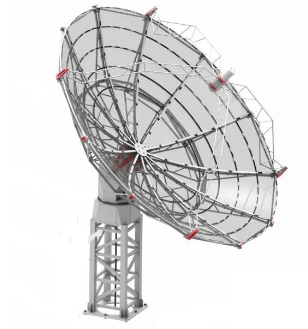
\includegraphics[height = 8cm ]{Figuras/seccion_1/antena_MIA.png}
	\caption{Antena en proceso de construcción para interferómetro MIA}
	\label{fig:antena_mia}
\end{figure}


En el caso del interferómetro, se trata de una nueva tecnología hasta ahora inexistente en el observatorio y permitiría incrementar la capacidad científica, tecnológica y observacional del Instituto; mientras que la estación terrena, permitirá establecer enlaces de comunicación con pequeños satélites como parte de las actividades del IAR en el segmento aeroespacial.

Actualmente el posicionador que se ha desarrollado se encuentra instalado pero tiene la limitación de funcionar con un solo programa (Gpredict), y no puede realizar el seguimiento de radiofuentes. A este software se deben agregar estas radiofuentes, o adicionarle la comunicación con otro software de seguimiento, para que funcione, y es de operación manual. Actualmente sigue en estado de prototipo.  

Se desea realizar un nuevo posicionador sin las limitaciones que posee el prototipo mencionado en el párrafo anterior. En este posicionador se busca que los scripts desarrollados para el manejo de las antenas principales estén embebidos en el sistema y se comuniquen con los programas Gpredict y Stellarium. Se desea agregar escalabilidad al software para que si se desea adicionar otro programa (por ejemplo Orbitron), el software se pueda escalar fácilmente.      
%Se desea mejorar incluyendo independencia de software, o mecanismos de manejo remoto, mediante protocolos existentes para las antenas principales. En la figura \ref{fig:antenas_main} se muestran las dos antenas principales del organismo. 

%% 
El sistema de apuntamiento, debe realizar el seguimiento automático (de posición astronómica) de los puntos del cielo, ya sean satélites o radiofuentes. En el caso de no realizar seguimientos, debe permanecer en la posición denominada cenit. En este caso, el sistema debe estar a lazo cerrado todo el tiempo, siguiendo una referencia, que viene dada por una computadora/software, dentro de ciertos márgenes. 
Adicionalmente, al estar en un lugar remoto dentro del organismo, debe poseer telemetria, ya que pueden existir condiciones climaticas adversas en las cuales la antena no podría operarse (por ejemplo, viento, granizo, ya que en estos casos, la antena actúa como una vela de barco). En la Figura \ref{fig:bloques_sistema}  se presenta el diagrama en bloques del sistema a realizar. 
%imagen de la antena % 

\begin{figure}[h]
	\vspace{-0.05cm}
	\centering
	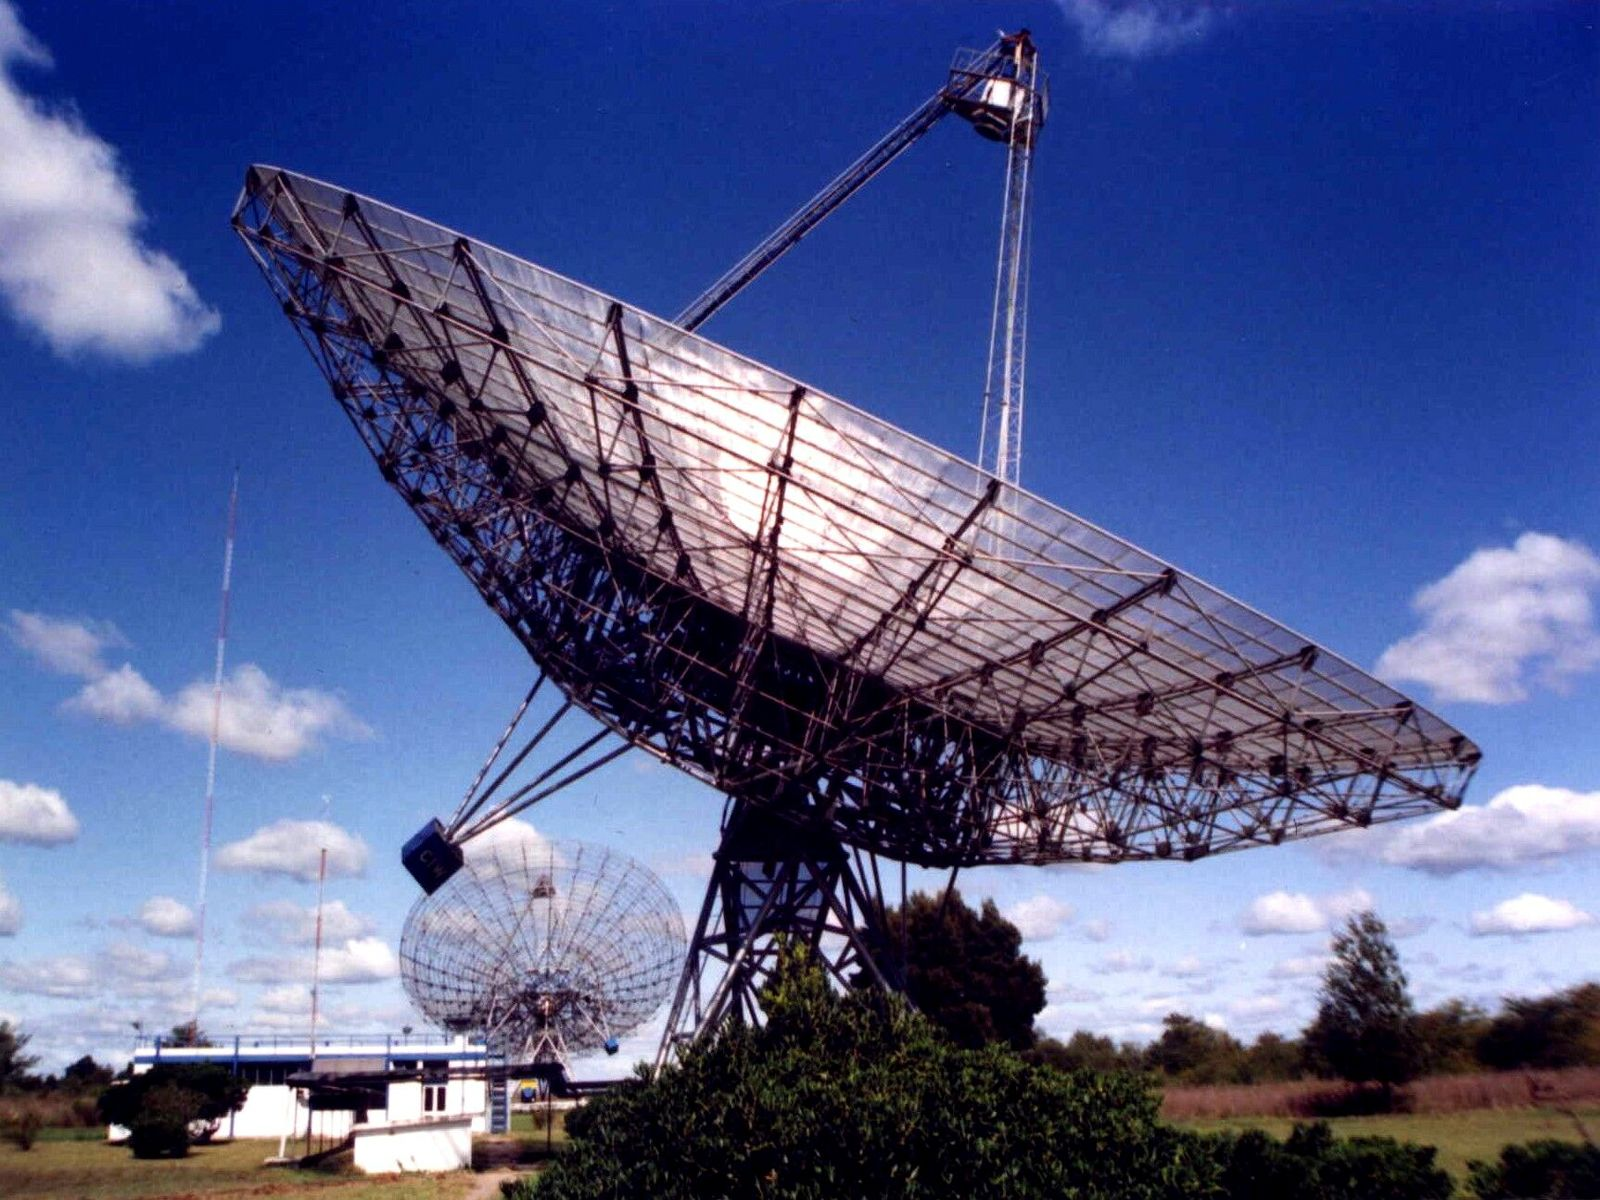
\includegraphics[scale = 0.2]{Figuras/seccion_1/antena_main.jpg}
	\caption{Antenas principales del IAR}
	\label{fig:antenas_main}
\end{figure}

\begin{figure}[h!]
	\vspace{-0.1cm}
	\centering 
	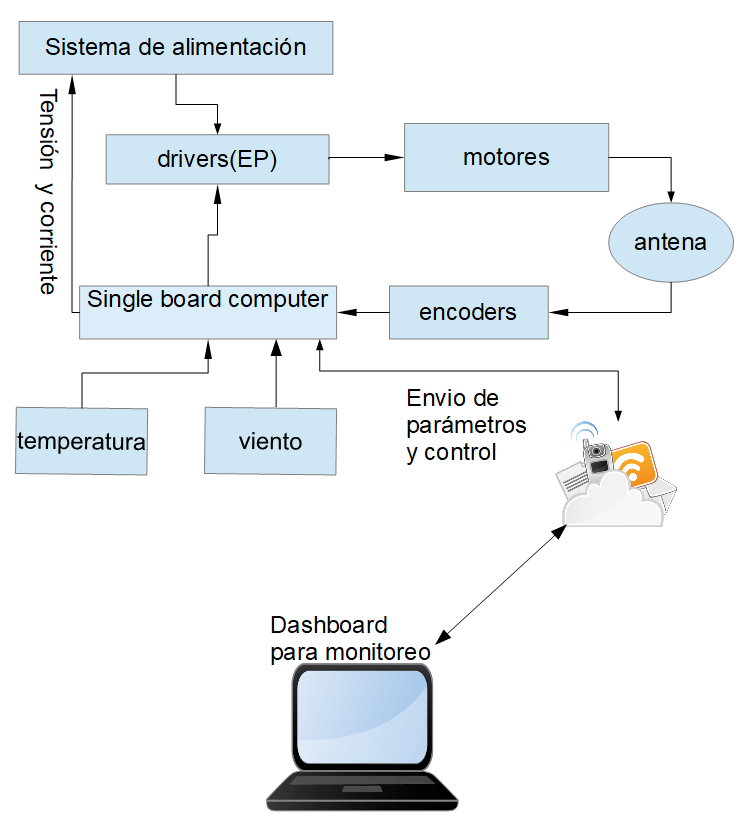
\includegraphics[height=11cm,width =\textwidth]{Figuras/seccion_1/interferometria.png}
	\caption{Diagrama en bloques del sistema }
	\label{fig:bloques_sistema}
\end{figure} 



\section{2. Identificación y análisis de los interesados}
\label{sec:interesados}

\begin{table}[ht]
%\caption{Identificación de los interesados}
%\label{tab:interesados}
\renewcommand {\arrayrulewidth}{1pt}
\begin{tabularx}{\linewidth}{@{}|l|X|X|l|@{}}
	\hline
	\rowcolor[HTML]{C0C0C0} 
	Rol           & Nombre y Apellido & Organización 	& Puesto 	\\ \hline
	Auspiciante   & -                 &  -             	& -        	\\ \hline
	Cliente       & -  			      &	 -				& -       	\\ \hline
	Impulsor      &  -                & -             	& -       	\\ \hline
	Responsable   & \authorname       & IAR        	    & Ing desarrollo firmware/hardware 	\\ \hline
	Colaboradores & Martín Salibe     & IAR             & Responsable de transferencia \\
				  &  Guillermo Gancio & IAR             & Responsable de observatorio \\ \hline
	Orientador    & \supname	      & \pertesupname 	& Director Trabajo final \\ \hline
	Equipo        & Eliseo Diaz \newline 
	Matias Contreras          & IAR              	& Responsables de fabricación de PCB y 3D  	\\ \hline
	Opositores    &  -                 & -             	& -        	\\ \hline
	Usuario final & Facundo Aquino     & IAR           	& Operador de antena  y diseñador PCB    	\\ \hline
\end{tabularx}
\end{table}




\section{3. Propósito del proyecto}
\label{sec:proposito}
	El propósito de este proyecto es realizar un sistema de apuntamiento para una antena (ver figura \ref{fig:antena_mia}). Esta antena debe ponerse en el cenit en caso de no realizar ningún tipo de seguimiento, ya que este punto es el de equilibrio mecánico. Una vez finalizado este desarrollo, se lo replicará en otras tres antenas de iguales características. 


\section{4. Alcance del proyecto}
\label{sec:alcance}
El proyecto tendrá el siguiente alcance: 
\begin{itemize}
	\item Desarrollo de firmware/software/hardware para realizar el movimiento de los motores de posición. 
	\item  Documentación de software/firmware/hardware por separado.
	\item  Desarrollo del protocolo de comunicación entre encoders y PC.
	\item  Integración del producto con el sistema mecánico de movimiento.
	\item Planes de testing para software y hardware. 
	
\end{itemize}

El proyecto no contempla aspectos relacionados a la seguridad de la información, y a la selección de los motores para el posicionamiento.  


\section{5. Supuestos del proyecto}
\label{sec:supuestos}
	Para el desarrollo se supone que se tiene acceso a los siguientes items: 
	\begin{itemize}
		\item Máquina con sistema operativo linux o similar. 
		\item Los recursos de hardware y software se proveen por la institución, así como su documentación.
		\item Se tiene acceso a los desarrollos previos realizados para el control de la antena. 
		\item El sistema mecánico se debe armar antes de octubre/noviembre 2022, que esta a cargo del departamento de mecánica. En caso de no realizarse, se verá la forma de simular en algún tipo de software. 
		\item El proyecto está inmerso dentro de un plan estratégico dentro de la institución. 
		\item Los componentes se encuentran en el mercado local, y en el caso de importarse, se realizará con la suficiente antelación. 
		\item La estructura mecánica de movimiento de la antena estará lista antes de la finalización del presente proyecto. 
		\item Existe disponibilidad para la utilización del router CNC para fabricar PCBs, en caso de que fuera necesario. 
		\item El personal abocado al diseño mecánico realizará el trabajo en tiempo y forma.  
		\item El proyecto se seguirá enmarcando dentro de un plan estratégico para la institución.  
		\item No va a cambiar la prioridad del proyecto del personal asignado al mismo.  
 

	\end{itemize}
	


\section{6. Requerimientos}
\label{sec:requerimientos}

\begin{enumerate}
	\item Requerimientos funcionales
		\begin{enumerate}
			\item Debe tener un sistema de control de posición en dos ejes (azimuth y altura).
			
			\item Debe poseer un Webserver embebido para monitoreo de variables ambientales e indicar su estado de operación (tracking, untracking, zenit, y calibrate). 
			\item Debe implementarse lecturas de posicionamiento, lecturas de viento, temperatura y potencia consumida por el mismo. 
			\item Debe conectarse a red local LAN, mediante cable ethernet RJ45. 
			
			\item Debe detener su funcionamiento cuando el viento sea superior a 50 km/h durante al menos 10 minutos y volver a su posición de equilibrio mecánico (cenit) 
			\item Debe tener un sistema de calibración a demanda por el operario de la antena. 
			\item El software se debe conectar con los programas Gpredict, Stelarium y el existente en el IAR para el manejo de las antenas principales. 
			\item El software debe manejar los periféricos del single board computer. 
			\item El software debe permitir la lectura de viento (velocidad en km/h), tensión , corriente en Ampere y posición angular (en grados) de la antena en ambos ejes. 
			\item El software realizará un reporte diario a las 5 AM con todos los datos almacenados en formato csv.  
			\item En caso de adicionar otro programa distinto al Gpredict, Stellarium o los scripts existentes en el IAR, se debe actualizar el software del sistema posicionador. 
			\item Solo puede realizar una operación de seguimiento. En caso de estar realizando el seguimiento de algún satelite/radiofuente, se le debe informar de dicha operación, y el operario tendrá que esperar que se termine la operación actual.  
			\item Debe poseer un control de velocidad para realizar el seguimiento.
			\item Los encoders deben tener una resolucion menor a diez veces el ancho de haz de antena (aproximadamente 0.2 º).
		\end{enumerate}
	\item Requerimientos de documentación
		\begin{enumerate}
			\item Debe seguir la numeración y formato de los documentos establecidos por el IAR. 
			\item Documentación sobre protocolos de comunicación via ethernet y de los programas involucrados y trama de mensajes.
			\item Manual de operación de la antena para operarios. 
			\item Manual de operación para actualización de software. 
			\item Documentación de software y hardware. 
			\item Manual de procedimientos de testing de software y hardware.	
			\item Reporte de test de software y hardware. 
			\item Descripción del sistema a la respuesta al escalón y función de transferencia
	\end{enumerate}
	\item Requerimientos de interfaces
		\begin{enumerate}
			\item Los encoders estarán alineados con los dos ejes principales de movimiento de la antena. 
			\item Deberá utilizarse una red electrica para conectar el posicionador.
		\end{enumerate}
	\item Requerimiento de testing
		\begin{enumerate}
			\item Medir señal de control de posición de los motores.
			\item Webserver embebido, testing de señales sobre la placa con osciloscopio.
			\item Realizar el seguimiento de una radiofuente, e intentar realizar más de una conexión simultanea. 
			\item Ver la señal de control mínima a partir de la cual los motores son capaces de mover la antena. 
			\item Podría realizase una experiencia de rebote lunar con Stellarium (esto ya se ha realizado con anterioridad con las antenas principales de la institución). El objetivo es corroborar la calibración del mismo y la comunicación con el software.  

		\end{enumerate}
\end{enumerate}

\section{7. Historias de usuarios (\textit{Product backlog})}
\label{sec:backlog}

Las historias de usuario, se realizan desde la perspectiva del operador de antena y el responsable de observatorio. Estas historias contempladas en esta sección se evalúan en base a su complejidad de realización y el criterio seleccionado es el siguientes: 
\begin{itemize}
	\item Muy bajo: 1 puntos. 
	\item Bajo: 2 puntos.
	\item Medio: 3 puntos. 
	\item Alto: 4 puntos. 
	\item Muy alto: 5 puntos.
\end{itemize}

\begin{itemize}
	\item Como operador debería tener telemetría para visualizar el estado de los instrumentos receptores y la radiofuente seguida por la antena abandonando la terminal de Linux. 
		\begin{itemize}
			\item Medio: 4 puntos.
		\end{itemize}

	\item Los operadores de antena deberían poder moverla mediante una interfaz de usuario. 
		\begin{itemize}
			\item Alto: 4 puntos.
		\end{itemize}
	
	\item Los operadores de antena deben tener el mayor control de configuración sobre los parámetros de la antena (posición, temperatura, viento, ajuste de tensiones, movimiento manual, control de receptores,etc). 
		\begin{itemize}
			\item Muy alto: 5 puntos.
		\end{itemize}
		

\end{itemize}

%Considerando la suma de las tres puntuaciones, se puede decir que hay 13 puntos de dificultad 
% 



\section{8. Entregables principales del proyecto}
\label{sec:entregables}



Los entregables princiapales del proyecto son:

\begin{itemize}
	\item Manual de uso. 
	\item Diagrama de circuitos esquemáticos si los hubiera. 
	\item Código fuente del firmware. 
	\item Manual de actualización del firmware.  
	\item Manual de procedimientos de testing de software y hardware.
	\item Manual de operación de la antena. 
	\item Descripción del sistema a la respuesta al escalón y función de transferencia (descripción breve con resultados relevantes).
	\item Informe final.
\end{itemize}



\section{9. Desglose del trabajo en tareas}
\label{sec:wbs}

\begin{enumerate}
\item Investigación preliminar (59 hs): 
	\begin{enumerate}
	\item Búsqueda bibliográfica sobre sistemas de coordenadas y control digital (5 hs). 
	\item Investigación de sistemas de coordenadas astronómicas y su transformación matemática (10 hs). 
	\item Selección del microcontrolador/single board computer y generación de tabla comparativa (10 hs).  
	\item Instalación de herramientas de desarrollo y documentación (8 hs).
	\item Estudio del manejo de periféricos de la placa seleccionada (15 hs).
	\item Análisis del hardware disponible en mercado local e internacional (8 hs).
	\item Primer informe de avance (3 hs).  
	\end{enumerate}
\item Diagramas de software (34 hs): 
	\begin{enumerate}
		\item Diagrama de software para módulos de lectura de sensores (3 hs).  
		\item Diagrama de software para el control de posición (5 hs). 
		\item Diagrama de software para integración de lectura de sensores y control de posición (8 hs) . 
		\item Creación de interfaz de usuario para el webserver embebido (4 hs).
		\item Creación de interfaz de usuario para el posicionamiento manual (4 hs).
		\item Diagrama de integración de los módulos de software (5 hs). 
		\item Generación parcial de documentación de software y hardware (5 hs).
	\end{enumerate}
\item Desarrollo de software para lectura de sensores (53 hs) :
	\begin{enumerate}
	\item Modulo de lectura del anemómetro (15 hs). 
	\item Modulo de lectura de la tensión y corriente (10 hs). 
	\item Módulo de lectura de encoders(10 hs). 
	\item Módulo de armado de archivo csv y envió cada 24 hs de la telemetría (8hs).
	\item Testing de software y generación de informe parcial (8 hs). 
	\item Informe de avance(2hs). 		
	\end{enumerate}
\item Desarrollo del control de posición (105 hs):  
	\begin{enumerate}
	\item  Desarrollo de herramientas de software/hardware para generar escalones de tensión y medir posición (30 hs). 
	\item  Generación de informe de respuesta al escalón (25 hs). 
	\item  Desarrollo del software de control digital (30 hs).  
	\item  Testing del control mediante simulación manual del encoder o sobre la antena(dependiendo de si se ha construido o no la antena) (10hs).   
	\item  Reporte de resultados del testing (10 hs). 	
\end{enumerate}
\item Desarrollo del webserver (200 hs):  
	\begin{enumerate}
		\item Instalación del servidor web(30 hs).
		\item Creación del sistema de consulta de estado (25 hs). 
		\item Programación del webserver con la interfaz (25 hs). 
		\item Integración de interfaz con el control de posición y lectura de sensores (35 hs). 
		\item Creación de API de consulta (30 hs). 
		\item Generación de informe parcial de manual de operación de antena mediante webserver (20 hs). 
		\item Generación parcial de documentación de software y hardware (10 hs).  
	\end{enumerate}
\item Desarrollo de conexión con Gpredict, Stellarium y scripts del IAR (58 hs):
	\begin{enumerate}
		\item Modulo de software para conexión con Gpredict (8 hs).
		\item Módulo de software para conexión con Stellarium (20 hs). 
		\item Módulo de software desarrollado en el IAR compatible con las antenas principales (25 hs). 
		\item Generación de documentación sobre protocolos de comunicación via ethernet y trama de mensajes (5 hs). 
	\end{enumerate}
\item Módulo de actualización de software (70 hs): 
	\begin{enumerate}
		\item Desarrollo de módulo de actualización de software (30 hs). 
		\item Testing de actualización de software (20 hs) . 
		\item Manual de actualización de software (10 hs).
		\item Generación de la documentación sobre software y hardware (10 hs).
		  
	\end{enumerate}	
\item Integración de los sistemas y ensamblado (169 hs): 
	\begin{enumerate}
	\item Ordenamiento de sistemas de información (3 hs). 
	\item Integración de los módulos de software (39 hs)
	\item Construcción del plan de pruebas (3 hs). 
	\item Desarrollo del plan de pruebas (24 hs). 
	\item Generación de reporte del plan de pruebas y resultados (10 hs).  
	\item Desarrollo de shield o escudo para la placa seleccionada (15 hs). 
	\item Testing con operadores de antena del IAR (40 hs). 
	\item Reporte de resultados de operadores de antena del IAR y posibles mejoras (30 hs).
	\item Montaje final en lugar de operación (5 hs).
	\end{enumerate}	
\item Generación de documentación (95 hs)
	
	\begin{enumerate}
	\item Completar la documentación de software y hardware (30 hs).
	\item Memoria técnica y construcción de diapositivas para presentación(40 hs). 
	\item Reportes de resultados de observaciones y adjuntarlas como anexo al documento final(25 hs). 
	\end{enumerate}
	

\end{enumerate}
	
Cantidad total de horas :  843 hs  



\section{10. Diagrama de Activity On Node}
\label{sec:AoN}
El diagrama de Activity on Node se muestra en la figura \ref{fig:AoN} y el código de colores que se usa en el diagrama se muestra a continuación: 
\begin{figure}[H]
	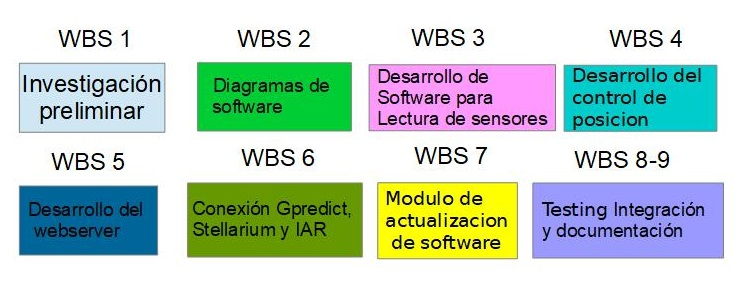
\includegraphics[width = \textwidth,height = 5.1cm]{./Figuras/AonGantt/cod_colores.jpg}
	\caption{Código de colores utilizado en el diagrama de la figura \ref{fig:AoN}}
\end{figure} 

\begin{figure}[H]
\centering
%[width = \textwidth, height = 15cm]
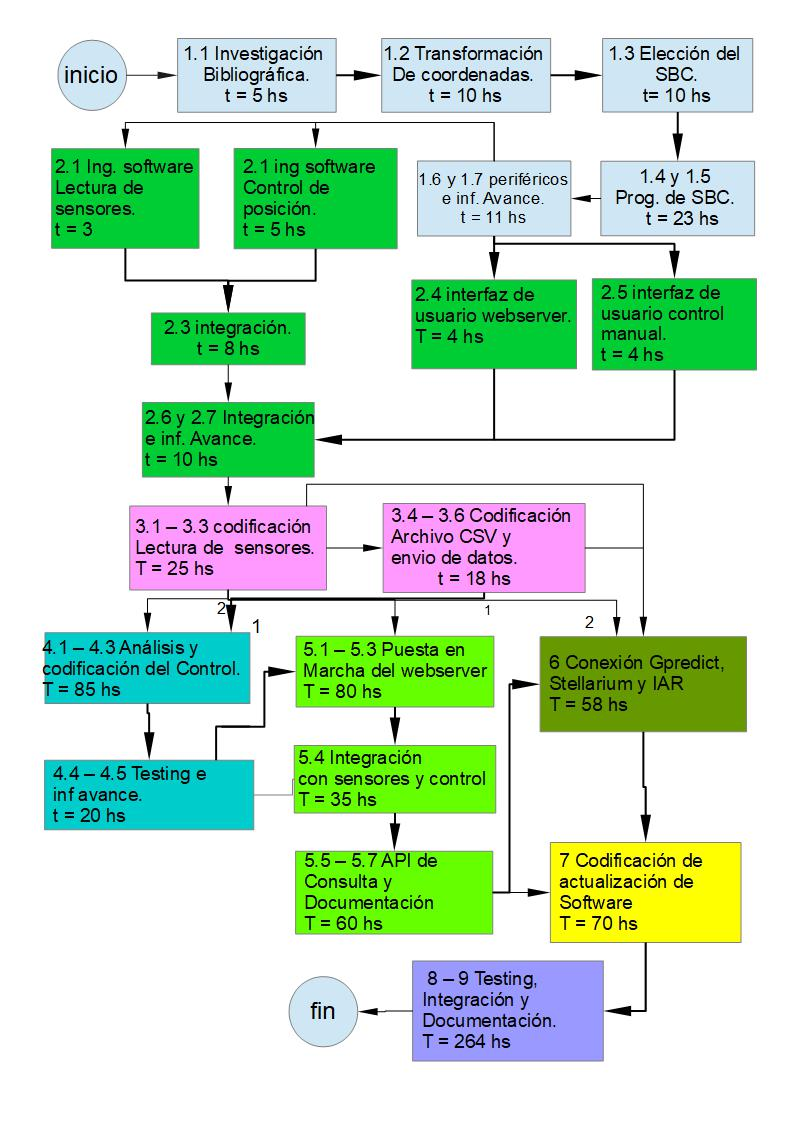
\includegraphics[width = \textwidth, height = 17cm]{./Figuras/AonGantt/ActivityOnNode.jpg}
\caption{Diagrama de \textit{Activity on Node}}
\label{fig:AoN}
\end{figure}

\section{11. Diagrama de Gantt}
\label{sec:gantt}
El diagrama de Gantt se muestra en la figura \ref{fig:diaGANTT}, habiéndose estimando unas 30 hs de trabajo semanales. Se han contemplado días festivos y feriados de la República Argentina. 


\begin{figure}[H]
	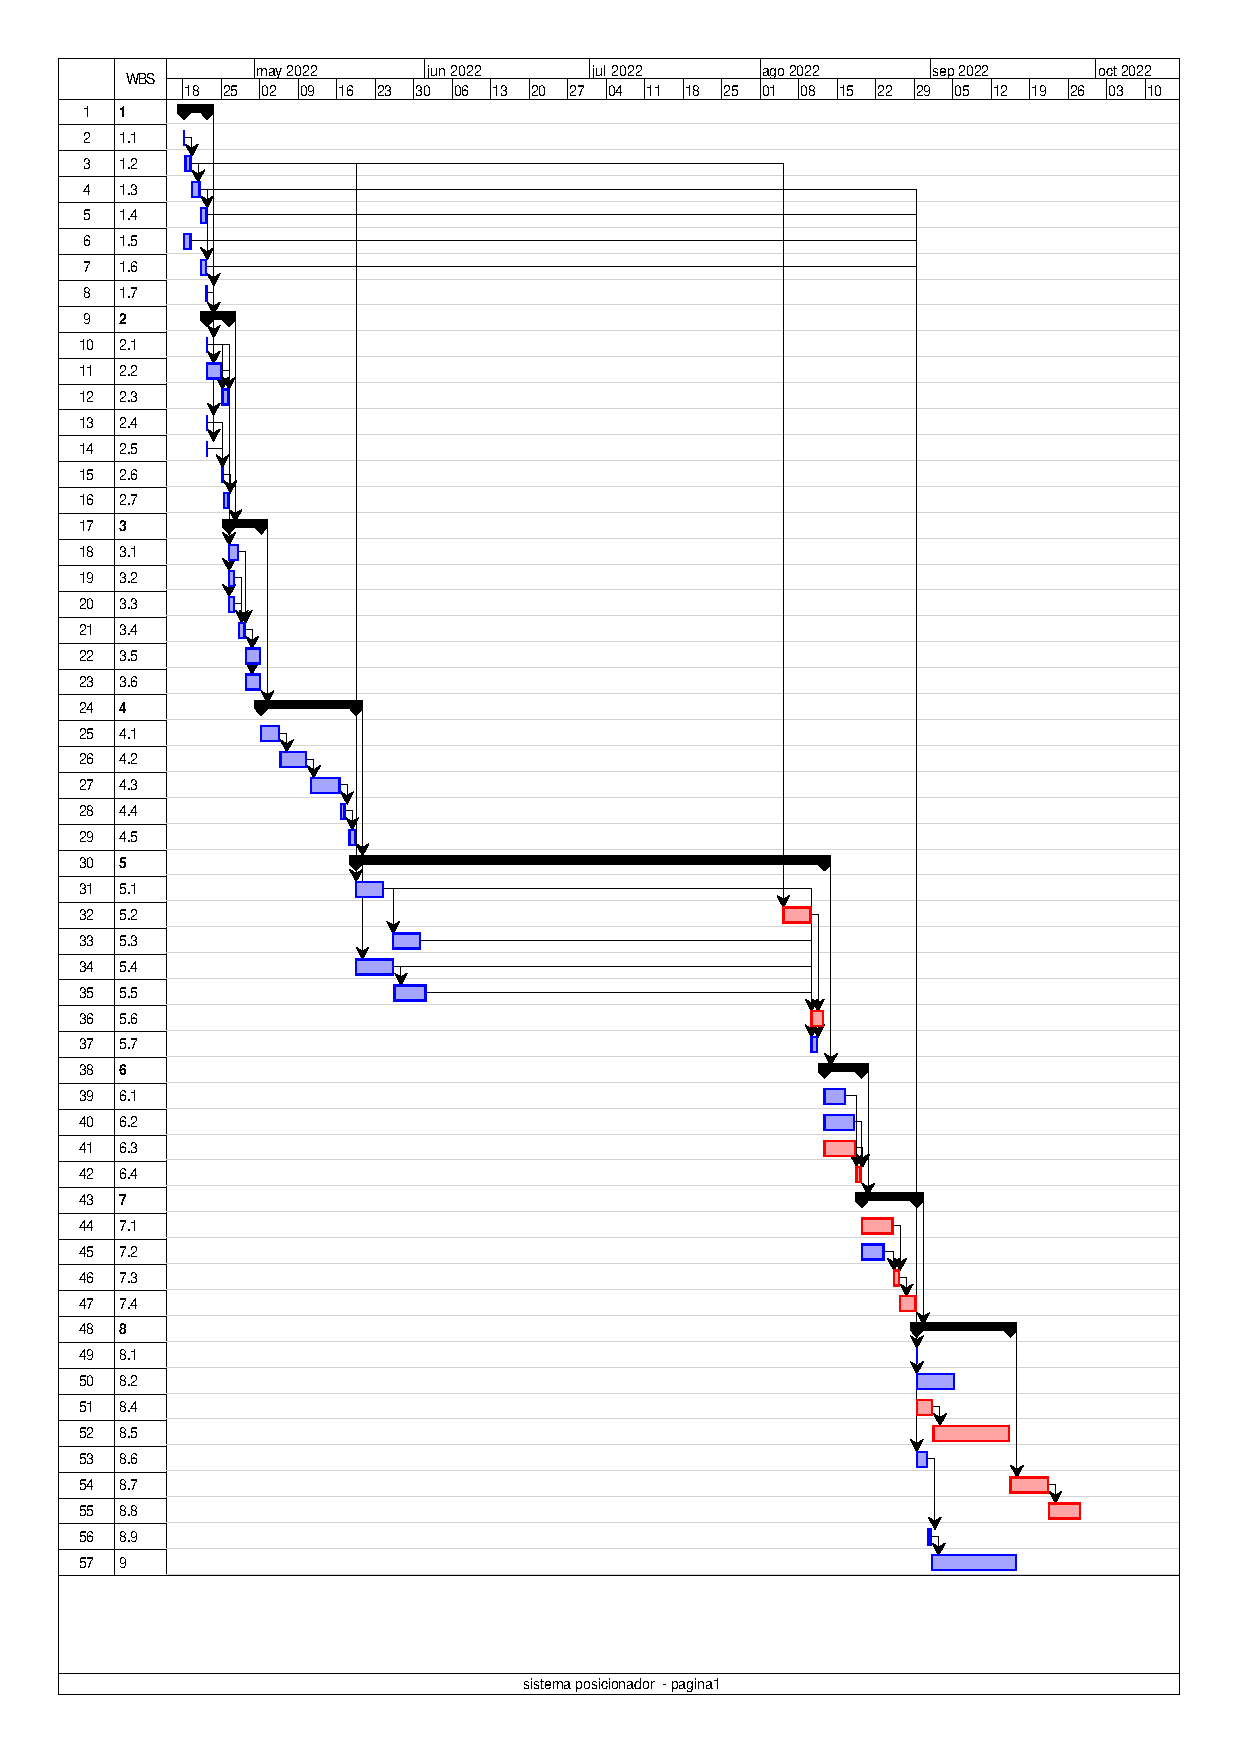
\includegraphics[width = \textwidth, height = 21.2cm,trim={0 3cm 0  0.1cm},clip ]{./Figuras/AonGantt/gannt_poss.pdf}
	\caption{Diagrama de gannt estimado del proyecto}
	\label{fig:diaGANTT}
\end{figure}




\section{12. Presupuesto detallado del proyecto}
\label{sec:presupuesto}
El presupuesto es estimativo porque el desarrollo del producto no se ha iniciado. Los componenentes adquiridos a la fecha son los encoders absolutos, presentados en la tabla de presupuestos. 
\def\tablename{Tabla}%
%El resto del presupuesto aún no se ha definido de forma detallada dado que el desarrollo no se ha iniciado aún. 
\begin{table}[htpb]
\centering
\begin{tabularx}{\linewidth}{@{}|X|c|r|r|@{}}
	\hline
	\rowcolor[HTML]{C0C0C0} 
	\multicolumn{4}{|c|}{\cellcolor[HTML]{C0C0C0}COSTOS DIRECTOS} \\ \hline
	\rowcolor[HTML]{C0C0C0} 
	Descripción &
	  \multicolumn{1}{c|}{\cellcolor[HTML]{C0C0C0}Cantidad} &
	  \multicolumn{1}{c|}{\cellcolor[HTML]{C0C0C0}Valor unitario} &
	  \multicolumn{1}{c|}{\cellcolor[HTML]{C0C0C0}Valor total} \\ \hline
   Single board computer&
  \multicolumn{1}{c|}{2} &
  \multicolumn{1}{c|}{20000} &
  \multicolumn{1}{c|}{40000} \\ \hline
 anemómetro o construcción del mismo &
 \multicolumn{1}{c|}{1} &
 \multicolumn{1}{c|}{30000} &
 \multicolumn{1}{c|}{30000} \\ \hline
 Encoders absolutos AMT20
   & \multicolumn{1}{c|}{2}
   & \multicolumn{1}{c|}{20000}
   & \multicolumn{1}{c|}{50000}   \\ \hline
   Diseño puente H   
   & \multicolumn{1}{c|}{2}
   & \multicolumn{1}{c|}{15000}
   & \multicolumn{1}{c|}{30000}
   \\ \hline
   Sensores de tensión y corriente
   & \multicolumn{1}{c|}{6}
   & \multicolumn{1}{c|}{500}
   & \multicolumn{1}{c|}{3000}
   \\ \hline
   \multicolumn{3}{|c|}{SUBTOTAL} &
   \multicolumn{1}{c|}{153000} \\ \hline
   \rowcolor[HTML]{C0C0C0} 
   \multicolumn{4}{|c|}{\cellcolor[HTML]{C0C0C0}COSTOS INDIRECTOS} \\ \hline
   \rowcolor[HTML]{C0C0C0} 
   Descripción &
  \multicolumn{1}{c|}{\cellcolor[HTML]{C0C0C0}Cantidad} &
  \multicolumn{1}{c|}{\cellcolor[HTML]{C0C0C0}Valor unitario} &
  \multicolumn{1}{c|}{\cellcolor[HTML]{C0C0C0}Valor total} \\ \hline
Elementos de ferreteria(tornillos, conectores, cables, cajas estancas,etc) 
& \multicolumn{1}{c|}{-}
& \multicolumn{1}{c|}{-}
& \multicolumn{1}{c|}{5000}   \\ \hline
Circuitos integrados y electrónica discreta
& \multicolumn{1}{c|}{-}
& \multicolumn{1}{c|}{-}
& \multicolumn{1}{c|}{10000}   \\ \hline
Gastos extra de impresoras 3D y CNC (fresa, extrusor, etc)  
& \multicolumn{1}{c|}{-}
& \multicolumn{1}{c|}{-}
& \multicolumn{1}{c|}{10000}   \\ \hline
\multicolumn{3}{|c|}{SUBTOTAL} &
\multicolumn{1}{c|}{25000} \\ \hline 
\rowcolor[HTML]{C0C0C0} 
\multicolumn{3}{|c|}{TOTAL} &
\multicolumn{1}{c|}{178000} \\ \hline

%\multicolumn{3}{|c|{TOTAL} &
%\multicolumn{1}{c|}{} \\ \hline
%

\end{tabularx}%

\caption{Tabla de costos directos e indirectos en base a estimaciones iniciales del proyecto}
\end{table}


\section{13. Gestión de riesgos}
\label{sec:riesgos}

Riesgo 1: El sistema mecánico de movimiento de la antena no esté listo antes de la tarea 4.
\begin{itemize}
	\item Severidad(S): 8.\newline
		La severidad es alta dado que el objetivo principal del trabajo es realizar el control sobre ella.
	\item Probabilidad de ocurrencia (O): 3. \newline
	 Se asigna esta probabilidad dado que se han comprado los materiales estructurales para su construcción. Cabe destacar que su construcción esta a cargo del departamento de mecánica. 
\end{itemize}

Riesgo 2: Que el proyecto deje de estar entre los objetivos estratégicos de la institución.
\begin{itemize}
	\item Severidad(S): 8.\newline
	La severidad es alta dado que el proyecto no se terminaría en tiempo y forma pactada. Además, se asignarían los recursos del presente proyecto a otro. 
	\item Probabilidad de ocurrencia (O): 3. \newline
	Esta probabilidad se asigna dado que una de las funciones principales es la observación del espacio mediante ondas de radio.  
\end{itemize}


Riesgo 3: Realizar mal la estimación de duración de las tareas. 
\begin{itemize}
	\item Severidad(S): 7.\newline 
	Se asigna esta puntuación debido a que se demora el prototipo funcional para solicitar nuevas fuentes de financiamiento y colaboraciones de radiotelescopios internacionales.
	\item Probabilidad de ocurrencia (O): 7.\newline 
	Alta, debido a que hay tareas a las cuales no se tiene experiencia.
\end{itemize}


Riesgo 4: No conseguir los componentes para realizar el rebote lunar. 
\begin{itemize}
	\item Severidad(S): 4.\newline 
		Si bien es deseable su realización, no afecta al funcionamiento del proyecto ni su objetivo principal. 
	\item Probabilidad de ocurrencia(O): 4.\newline 
		La probabilidad es baja porque existen los componentes y el personal calificado para llevarlo a cabo. 
\end{itemize}

Riesgo 5: Algunos de los componentes no se encuentren en el mercado local. 
\begin{itemize}
	\item Severidad(S): 4.\newline 
		Si los componentes deben importarse, implica un retraso importante en el proyecto dado que se tendrá que trabajar con placas ya existentes en el laboratorio. 

	\item Probabilidad de ocurrencia (O): 7. \newline 
	   Se plantea que la mayor parte de los componentes se encuentren en el mercado local. En caso contrario, se verá la forma de mitigar este efecto, dado que al ser una institución del estado nacional, las compras en el extranjero se fijan por ROECYT y tiene una duración estimada de 6 meses aproximadamente. 
\end{itemize}





b) Tabla de gestión de riesgos:      (El RPN se calcula como RPN=SxO)

\begin{table}[htpb]
\centering
\begin{tabularx}{\linewidth}{@{}|X|c|c|c|c|c|c|@{}}
\hline
\rowcolor[HTML]{C0C0C0} 
Riesgo & S  & O  & RPN & S*  & O* & RPN* \\ \hline
   1   & 8  & 3  &  24 & 5   & 2  & 10     \\ \hline
   2   & 8  & 3  &  24 & 2   & 2  &  4    \\ \hline
   3   & 7  & 7  &  49 & 7   & 7  &  14   \\ \hline
   4   & 4  & 4  &  16 &     &    &      \\ \hline
   5   & 7  & 4  &  28 & 3   & 3  &  9    \\ \hline
   
\end{tabularx}
\end{table}

Se tomarán medidas de mitigación en los riesgos cuyos números de RPN sean mayores a 22 



Nota: los valores marcados con (*) en la tabla corresponden luego de haber aplicado la mitigación.

Plan de mitigación de los riesgos que originalmente excedían el RPN máximo establecido:
 
Riesgo 1: En caso que la estructura mecánica de la antena no se encuentre construida, hay dos antenas a escala para realizar el control. 
\begin{enumerate}
	\item Severidad (S): 5. \newline
	Si bien el control no es el mismo, se puede obtener el conocimiento sobre la forma de caracterizar sistemas de este tipo, para luego aplicarlo sobre las antenas originales del interferómetro MIA. Adicionalmente, se puede realizar un sistema de lazo cerrado sobre un banco de trabajo.   
	\item Probabilidad de ocurrencia(O): 2.\newline 
	Dado que los materiales para su construcción están comprados, no debería llegar a ocurrir. 
	
\end{enumerate} 

Riesgo 2: Se mostrarán las bondades del sistema de apuntamiento para volverlo a ubicar entre los objetivos estratégicos. 
\begin{itemize}
	\item Severidad (S): 2. \newline
	La institución entre sus objetivos principales es realizar mejoras sobre las antenas y su electrónica en forma continua 
	\item Probabilida de ocurrencia(O): 2. 
	Es díficil que ocurra porque existen proyectos de colaboración internacional. 
\end{itemize}





Riesgo 3: Se adicionaran horas hombre y se pedirá colaboración a los interesados.
\begin{itemize}
	\item Severidad (S): 7. \newline 
	Deberán sumar personal en caso de subestimación, y en caso de sobreestimación, no se corre ningún tipo de riesgo.
	\item Probabilidad de ocurrencia (O): 7.  \newline
	Debido al desconocimiento del estado del arte de algunas tareas por parte del diseñador del proyecto.  
\end{itemize}



Riesgo 5: Se iniciarán los desarrollos electrónicos contemplando el mercado local desde el origen del proyecto
\begin{itemize}
	\item Severidad (S): 3. \newline .
	Al iniciar el proyecto contemplando los componentes electrónicos en el mercado local disminuye su severidad. 
	\item Probabilidad de ocurrencia (O): 3.  \newline
	Dado que se contempla realizar las compras en el mercado local la probabilidad de ocurrencia disminuye. 
\end{itemize}




\section{14. Gestión de la calidad}
\label{sec:calidad}

\begin{enumerate}
\item Requerimientos funcionales 
	\begin{enumerate}
		\item Debe tener un sistema de control de posición en dos ejes (azimuth y altura).
				\begin{itemize}
					\item Verificación: se comprobará que el sistema de control responda ante una referencia de posición y colocando un receptor de banda L en la antena. 
					\item Validación: se entregará documentación sobre el sistema y modelado matemático del mismo. 
				\end{itemize} 
		
		\item Debe poseer un Webserver embebido para monitoreo de variables ambientales e indicar su estado de operación (tracking, untracking, zenit, y calibrate). 
			\begin{itemize}
				\item Verificación:se ingresará al webserver y se realizará un cambio de estado desde otra estación de trabajo. 
				\item Validación: se comprobará que el web server embebido no realice conexiónes con otras estaciones. Se entregará documentación sobre la operación a bajo nivel del mismo.  
			\end{itemize} 
%1.3		\item Debe implementarse lecturas de posicionamiento, lecturas de viento, temperatura y potencia consumida por el mismo. 
%1.4		\item Debe conectarse a red local LAN, mediante cable ethernet RJ45. 
		\setcounter{enumii}{4}	
%1.5 
		\item Debe detener su funcionamiento cuando el viento sea superior a 50 km/h durante al menos 10 minutos y volver a su posición de equilibrio mecánico (cenit) 
			\begin{itemize}
				\item Verificación: se girará el anemómetro mediante el acople a un motor de corriente continua durante 10 minutos. Luego se procede a intentará movilizar la antena. Se realiza una segunda prueba, pero ubicando la antena en una posición diferente del cenit. 
				\item Validación: se comprobará que la antena realice las maniobras correspondientes para regresar al cenit y no moverse. 
			\end{itemize} 
		\item Debe tener un sistema de calibración a demanda por el operario de la antena. 
			\begin{itemize}
				\item Verificación: se entregará un manual de operación de la antena para operarios.  
				\item Validación: Se comprobará que los operarios entiendan el manual de operación y se despejarán las dudas al respecto.   
			\end{itemize} 
		\item El software se debe conectar con los programas Gpredict, Stelarium y el existente en el IAR para el manejo de las antenas principales. 
			\begin{itemize}
				\item Verificación: se conectará con Gpredict y Stellarium, y se verificará un seguimiento completo.  
				\item Validación: se creará un manual de uso para los operarios de estos programas y se verificará que puedan realizar el seguimiento.   
			\end{itemize} 
		
%1 - 8 		\item El software debe manejar los periféricos del single board computer. 
% 1.9		\item El software debe permitir la lectura de viento (velocidad en km/h), tensión , corriente en Ampere y posición angular (en grados) de la antena en ambos ejes. 
% 1.10 		\item El software realizará un reporte diario a las 5 AM con todos los datos almacenados en formato csv.  
% 1. 11		\item En caso de adicionar otro programa distinto (Gpredict, stellarium o ya existente en el IAR) se debe actualizar el software del sistema posicionador. 
		\setcounter{enumii}{10}	
		\item Solo puede realizar una operación de seguimiento. En caso de estar realizando el seguimiento de algún satelite/radiofuente, se le debe informar de dicha operación, y el operario tendrá que esperar que se termine la operación actual.  
			\begin{itemize}
				\item Verificación: se procederá a realizar una operación de seguimiento desde una estación de trabajo, mientras la antena se encuentra en el estado de tracking.   
				\item Validación: se comprobará el rechazo e informe al operador de la segunda PC en cuestión al intentarse conectar y mover la antena.   
			\end{itemize} 
	\end{enumerate}

\item Requerimientos de documentación 
\begin{itemize}

	\item Verificación: Se completarán todos los entregables del proyecto sujeto a correcciones por parte de los miembros de la organización.  
	\item Validación: Se procede con el alta de documentación en el sistema SIGEVA del CONICET. 

\end{itemize}
\end{enumerate}




\section{15. Procesos de cierre}    
\label{sec:cierre}
\begin{enumerate}
	\item Análisis de seguimiento del plan original 
		\begin{itemize}
		\item Responsable: Gastón Valdez
		\item Actividades: 
			\begin{itemize}
				\item Se analizará el nivel de cumplimiento de los requerimientos.
				\item Comparación de fechas reales con la estimación del diagrama de gannt de la figura 	\ref{fig:diaGANTT}
			\end{itemize}
		\end{itemize}
	\item Identificación de procesos útiles e inútiles
		\begin{itemize}
			\item Responsable: Guillermo Gancio 
			\item Detectar de los procesos, cual de ellos puede repetirse o no en futuros desarrollos. 
		\end{itemize}
	\item Se dará agradecimiento a todos los interesados, y en especial al equipo de trabajo y
	colaboradores.
	\item Se realizará la presentación pública del proyecto, dando paso a la defensa del mismo ante jurados. 
	\item Se subirán los informes al servidor del instituto Argentino de Radioastronomía siendo aprobados por el director y codirector. 
\end{enumerate}



\end{document}
